\documentclass[11pt]{article}
\usepackage[a4paper,margin=1in]{geometry}
\usepackage{amsmath,amssymb,amsthm}
\usepackage{tikz}
\usepackage{xcolor}
\usepackage[hidelinks]{hyperref}
\hypersetup{pdftitle={Five numbers, many averages},pdfauthor={Vamshi Jandhyala}}
\setlength{\parskip}{0.4em}
\setlength{\parindent}{0pt}

\newtheorem{theorem}{Theorem}
\newtheorem{lemma}{Lemma}
\theoremstyle{remark}
\newtheorem*{remark}{Remark}

\definecolor{inkblue}{RGB}{40,76,105}
\definecolor{softblue}{RGB}{226,235,243}
\definecolor{rust}{RGB}{153,70,45}

\title{Five numbers, many averages}
\author{Vamshi Jandhyala}
\date{}

\begin{document}
\maketitle
\vspace{-2em}

\begin{abstract}
A move replaces two of a list of numbers by two copies of their average. We give, for every $k\ge1$, five
nonnegative integers that can be made equal by such moves, but by no fewer than $k+3$ of them. So for five
numbers there is no bound on the length of the shortest solution that depends only on how many numbers
there are. The lower bound comes from the dyadic weights that moves produce and from counting the entries
equal to the mean. Every step is checked in the Lean proof assistant.
\end{abstract}

\section{The question}

Take some numbers. A move picks two of them, $a$ and $b$, and replaces both by $(a+b)/2$. The mean never
changes, so the only possible end state is every number equal to the mean. Which lists can be brought there
in finitely many moves? The question was asked on MathOverflow~\cite{MO} and is open.

Some cases are easy. Two numbers take one move. Four numbers can be done in three: average two pairs, then a number
from each pair. The same doubling handles any power of two, and Shi, Li, Johansson and Johansson showed that
for any other count the generic list cannot be equalised~\cite{SLJJ16}. In the comments on the question Brendan
McKay noted that three numbers can be equalised exactly when they are in arithmetic progression, and that five
numbers can be when one of them already equals the mean: leave it alone and treat the other four as above.

Here is a list of five that has no entry equal to the mean $26$:
\[
(40,\,0,\,32,\,29,\,29).
\]
Stop and try to equalise it before reading on. It can be done in five moves (Figure~\ref{fig:moves}), and
it cannot be done in four. The example is the case $k=2$ of a family.

\begin{theorem}\label{thm:main}
Let $k\ge1$, $N=2^{k+1}$ and $\varepsilon=(-1)^k$. The five integers
\[
(5N,\;0,\;4N,\;3N+5\varepsilon,\;3N+5\varepsilon)
\]
can be made equal by pairwise averaging, and the least number of moves that does it is exactly $k+3$.
For $k\ge2$ no proper subset of them has the same mean as the whole.
\end{theorem}

So the shortest solutions for five numbers can be as long as we like, even for nonnegative integers and even
when no part of the list can be equalised on its own. A decision procedure for five numbers, if there is one,
has to look at the size of the numbers and not only at how many there are. The general question remains
open.

\begin{figure}[ht]
\centering
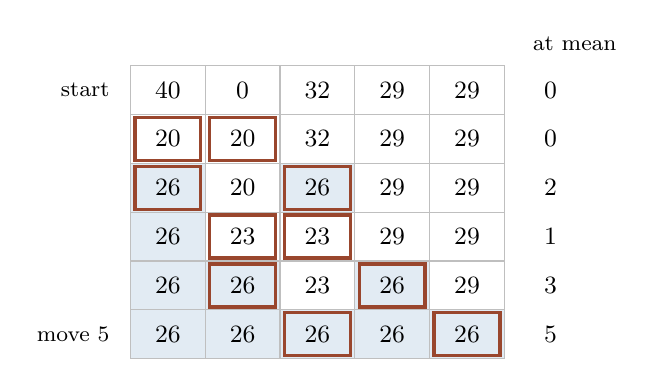
\begin{tikzpicture}[x=0.95cm,y=0.62cm]
  % the k = 2 example: rows are the states, the averaged pair outlined, entries equal to the mean shaded
  \foreach \r/\vals/\pa/\pb/\M in {
      0/{40,0,32,29,29}/-1/-1/0,
      1/{20,20,32,29,29}/0/1/0,
      2/{26,20,26,29,29}/0/2/2,
      3/{26,23,23,29,29}/1/2/1,
      4/{26,26,23,26,29}/1/3/3,
      5/{26,26,26,26,26}/2/4/5}{
    \foreach \v [count=\c from 0] in \vals {
      \ifnum\v=26 \fill[softblue] (\c,-\r) rectangle ++(1,-1); \fi
      \draw[gray!50] (\c,-\r) rectangle ++(1,-1);
      \node[font=\small] at (\c+0.5,-\r-0.5) {$\v$};
    }
    \ifnum\pa>-1
      \draw[rust,very thick] (\pa+0.06,-\r-0.06) rectangle ++(0.88,-0.88);
      \draw[rust,very thick] (\pb+0.06,-\r-0.06) rectangle ++(0.88,-0.88);
    \fi
    \node[font=\small,anchor=west] at (5.4,-\r-0.5) {$\M$};
  }
  \node[font=\footnotesize,anchor=west] at (5.25,0.45) {at mean};
  \node[font=\footnotesize,anchor=east] at (-0.15,-0.5) {start};
  \node[font=\footnotesize,anchor=east] at (-0.15,-5.5) {move 5};
\end{tikzpicture}

\caption{The case $k=2$: five moves equalise $(40,0,32,29,29)$. Each row is the list after a move; the two
entries that move changed are outlined, and entries equal to the mean $26$ are shaded. The right-hand column
counts them; it runs $0,0,2,1,3,5$. The count can only grow in steps of $2$ and can never be $4$, which is
why the last three moves cannot be saved (Lemma~\ref{lem:count}).}
\label{fig:moves}
\end{figure}

\section{A shrinking triple}

Moves commute with $x\mapsto cx+d$: averaging and then rescaling is the same as rescaling and then averaging.
So we may subtract $3N$ and divide by $N$, and work with
\[
B_k=\Bigl(2,\;-3,\;1,\;\tfrac52t,\;\tfrac52t\Bigr),\qquad t=\Bigl(-\frac12\Bigr)^{k},
\]
whose mean is $t$. The point of these numbers is a triple that can only creep towards its mean. Suppose three
entries are $(s,s,-2s)$, so that they sum to $0$. Average the odd one out with one copy of $s$:
\[
(s,\;s,\;-2s)\;\longmapsto\;\Bigl(-\frac s2,\;-\frac s2,\;s\Bigr).
\]
The shape is the same, with $s$ replaced by $-s/2$ (Figure~\ref{fig:triple}). Each move halves the distance
to $0$ and flips the sign.

\begin{figure}[ht]
\centering
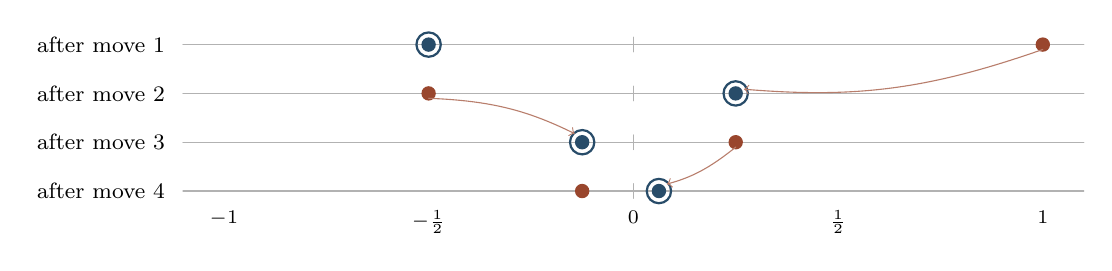
\begin{tikzpicture}[x=5.2cm,y=0.62cm,line cap=round]
  % rows: the first three entries after moves 1..4, as (s, s, -2s) with s = (-1/2)^m
  \foreach \m/\s in {1/-0.5,2/0.25,3/-0.125,4/0.0625}{
    \pgfmathsetmacro{\y}{-\m}
    \draw[gray!60] (-1.1,\y) -- (1.1,\y);
    \draw[gray!60] (0,\y-0.15) -- (0,\y+0.15);
    \pgfmathsetmacro{\d}{-2*\s}
    \fill[inkblue] (\s,\y) circle (2.6pt);
    \draw[inkblue,thick] (\s,\y) circle (4.4pt);
    \fill[rust] (\d,\y) circle (2.6pt);
    \node[left,font=\footnotesize] at (-1.12,\y) {after move \m};
  }
  \foreach \m/\s in {1/-0.5,2/0.25,3/-0.125}{
    \pgfmathsetmacro{\y}{-\m}
    \pgfmathsetmacro{\d}{-2*\s}
    \pgfmathsetmacro{\n}{-\s/2}
    \draw[->,rust!70,thin,shorten >=3pt] (\d,\y-0.1) to[bend left=12] (\n,\y-0.9);
  }
  \node[font=\scriptsize,below] at (0,-4.2) {$0$};
  \node[font=\scriptsize,below] at (1,-4.2) {$1$};
  \node[font=\scriptsize,below] at (-1,-4.2) {$-1$};
  \node[font=\scriptsize,below] at (0.5,-4.2) {$\tfrac12$};
  \node[font=\scriptsize,below] at (-0.5,-4.2) {$-\tfrac12$};
\end{tikzpicture}

\caption{The first three entries of $B_k$ after each move of the strategy: a repeated value $s$ (ringed) and
the odd one out $-2s$. Averaging the odd one out with a copy of $s$ gives the next row, with $s$ replaced by
$-s/2$.}
\label{fig:triple}
\end{figure}

\emph{The upper bound.} Average $2$ and $-3$: the first three entries become $(-\frac12,-\frac12,1)$, the
shape with $s=-\frac12$. After $k-1$ more moves of the triple they are $(t,t,-2t)$, and the list is
\[
\Bigl(t,\;t,\;-2t,\;\tfrac52t,\;\tfrac52t\Bigr).
\]
Average $-2t$ with one $t$, giving two copies of $-t/2$; then average each copy of $-t/2$ with one of the
$\frac52t$. Every entry is now $t$, after $k+3$ moves.

\section{Why there is no shortcut}

Two facts give the lower bound. The first says the mean is slow to appear, and the second says what happens
after it has.

\begin{lemma}[dyadic weights]\label{lem:weights}
After $r$ moves, each entry equals $\sum_i m_ix_i/2^r$, where $x_1,\dots,x_5$ are the starting numbers and
$m_1,\dots,m_5$ are nonnegative integers with $\sum m_i=2^r$.
\end{lemma}

\begin{proof}
At the start take $m$ to be $2^0=1$ at the entry itself and $0$ elsewhere. A move sends the weights of the
two averaged entries to their sum, over a denominator one power of $2$ larger; an entry not involved keeps its
value, which we rewrite with every $m_i$ doubled.
\end{proof}

\begin{lemma}[the mean is slow to appear]\label{lem:first}
Whatever the moves, no entry of $B_k$ equals $t$ before move $k$.
\end{lemma}

\begin{proof}
Scale by $N=2^{k+1}$: the list becomes $(2N,-3N,N,5\varepsilon,5\varepsilon)$ with mean $2\varepsilon$, since
$Nt=2\varepsilon$. Suppose an entry equals $2\varepsilon$ after $r<k$ moves. By Lemma~\ref{lem:weights},
\[
N\,(2m_1-3m_2+m_3)+5\varepsilon\,(m_4+m_5)=2^{r+1}\varepsilon .
\]
Multiply by $\varepsilon=\pm1$ and put $q=m_4+m_5$: then $5q-2^{r+1}=-\varepsilon N(2m_1-3m_2+m_3)$ is
divisible by $N=2^{k+1}$. Here $q$ is the total weight the entry gives to the two small inputs, and
$0\le q\le 2^r$. As $r<k$, $2^{r+1}$ divides $N$ and so divides $5q$, hence divides $q$; since $q<2^{r+1}$
this forces $q=0$. But then $N=2^{k+1}$ divides $2^{r+1}$, which is false for $r<k$.
\end{proof}

\begin{lemma}[counting entries at the mean]\label{lem:count}
Let $M$ be the number of entries equal to the mean. A move either does not increase $M$ or increases it by
exactly $2$, and $M$ is never $4$.
\end{lemma}

\begin{proof}
A move changes only the two entries $a,b$ it averages. If $(a+b)/2$ is not the mean, entries can leave the
mean but none join it. If $(a+b)/2$ is the mean and one of $a,b$ already equals it, so does the other, and
nothing changes. Otherwise both join, and $M$ grows by $2$. Finally, the five entries sum to five times the
mean, so if four of them equal the mean the fifth does too.
\end{proof}

\begin{proof}[Proof of Theorem~\ref{thm:main}]
The upper bound was shown in Section~2. For the lower bound, let a sequence of moves equalise $B_k$, and let
move $r_0$ be the first after which some entry equals $t$; by Lemma~\ref{lem:first}, $r_0\ge k$. Before it
$M=0$, so by Lemma~\ref{lem:count} $M=2$ just after it. The next move cannot raise $M$ to $4$, so leaves
$M\le2$; the one after leaves $M\le4$, hence $M\le3$. So $M=5$ needs at least three moves after move
$r_0$, and the sequence has at least $k+3$ moves.

For the last claim, let $k\ge2$, so $t\ne0$ and $-\frac18\le t\le\frac14$. No entry of $B_k$ equals $t$. The
pairs sum to $-1$, $3$, $-2$ (among the first three), $5t$ (the last two), or an integer plus $\frac52t$;
none of these is $2t$, because $2t$ is not an integer and $\frac52t+j=2t$ would need $j=-t/2$. A subset of
size three or four has mean $t$ exactly when its complement does, so no proper subset has mean $t$. The
case $k=1$ really is different: there $t=-\frac12$, and $2$ and $-3$ already average to $t$.
\end{proof}

\begin{remark}
Lemma~\ref{lem:first} is where the size of the numbers enters: the inputs of size $N$ and the inputs of
size $1$ can only be balanced by weights with a large power of $2$ in the denominator, and a large power of
$2$ takes many moves to make. Lemma~\ref{lem:count} is special to five numbers, where $M=4$ is ruled out by
the sum. Whether the solvable lists of five numbers can be recognised by a finite procedure is still open.
\end{remark}

\paragraph{Verification.} Every step of the proof of Theorem~\ref{thm:main} is checked in Lean~4 with Mathlib~\cite{mathlib}, using only
the standard axioms: the dyadic weights, invariance under affine maps and of the sum, Lemmas~\ref{lem:first}
and~\ref{lem:count}, the lower bound for every strategy, the explicit strategy of $k+3$ moves for every $k$,
the integer form and the claim about subsets. Python programs check the stated numbers in exact arithmetic,
including the least number of moves for small $k$ by complete search, and deliberately wrong variants fail
them; an independent program, sharing no code with the others, repeats the complete search. Everything is at
\url{https://github.com/jvvk/mathematics/tree/main/five-numbers-many-averages}.

\paragraph{Acknowledgements.} jh w asked the question on MathOverflow~\cite{MO}; the remarks in its comments
are credited above. Anthropic's Claude (Opus~5.5) was used to find the argument, write the Lean
formalisation and the programs, and draft this text. The author takes responsibility for the content.

\begin{thebibliography}{9}
\bibitem{MO} jh w, Make $n$ numbers equal using pairwise averages, MathOverflow question 421671 (3 May 2022),
\url{https://mathoverflow.net/q/421671}, accessed 10 October 2026.
\bibitem{SLJJ16} G.~Shi, B.~Li, M.~Johansson and K.~H.~Johansson, Finite-time convergent gossiping,
\emph{IEEE/ACM Trans. Networking} \textbf{24} (2016) 2782--2794,
\href{https://doi.org/10.1109/TNET.2015.2484345}{doi:10.1109/TNET.2015.2484345}.
\bibitem{mathlib} The mathlib Community, The Lean mathematical library, in \emph{Proceedings of the 9th ACM
SIGPLAN International Conference on Certified Programs and Proofs (CPP 2020)}, 367--381,
\href{https://doi.org/10.1145/3372885.3373824}{doi:10.1145/3372885.3373824}.
\end{thebibliography}

\bigskip
\noindent Vamshi Jandhyala, London, UK.

\end{document}
